\section{Introduction}
This chapter focuses on the overall presentation of our solution's architecture as well as that of the Apache Flink~\cite{FLINK} framework and Kubernetes~\cite{K8S}.
It highlights the key components of our system, how they interact and contribute to achieving our objective.

\section{Apache Flink framework overview}
Flink originates from the Stratosphere project, designed in 2008 by Professor Volker Markl and his team at the University of Berlin.
Flink has been one of the most important projects of the Apache Foundation since 2014.
In German, Flink means ``agile'' or ``fast'', like the squirrel in its logo.

Flink is an open-source framework for distributed processing of massive data.
It allows for efficient allocation and management of computing resources to run stream processing applications.
It integrates with all common cluster resource managers such as Hadoop YARN and Kubernetes, but can also be configured to operate as a standalone cluster or even as a library.
What makes it standout from others (such as Storm Hadoop MapReduce or Spark) is its native streaming API that offers extended functionalities.

\subsection{Technical architecture}
Flink operates and is deployed in a cluster of machines.
It works in a Master-Slave mode.
The master, called the JobManager, schedules tasks, distributes them to TaskManagers and tracks their execution progress.
It also allocates resources, and compiles results.
The slaves, called TaskManagers, execute the tasks sent by the JobManager and sometimes exchange data during different processing phases.
The core of the system lies in the processing engine (Runtime).
It can process data streams in streaming mode through the Stream Builder and the DataStream API as well datasets in batch mode with the batch optimizer and the DataSet API.
This execution engine is scalable and distributed, therefor enabling the processing of massive data (streaming or batch).
It also allows for the execution of iterative operations, memory management, and processing cost optimization.

\begin{center}
    \centering
    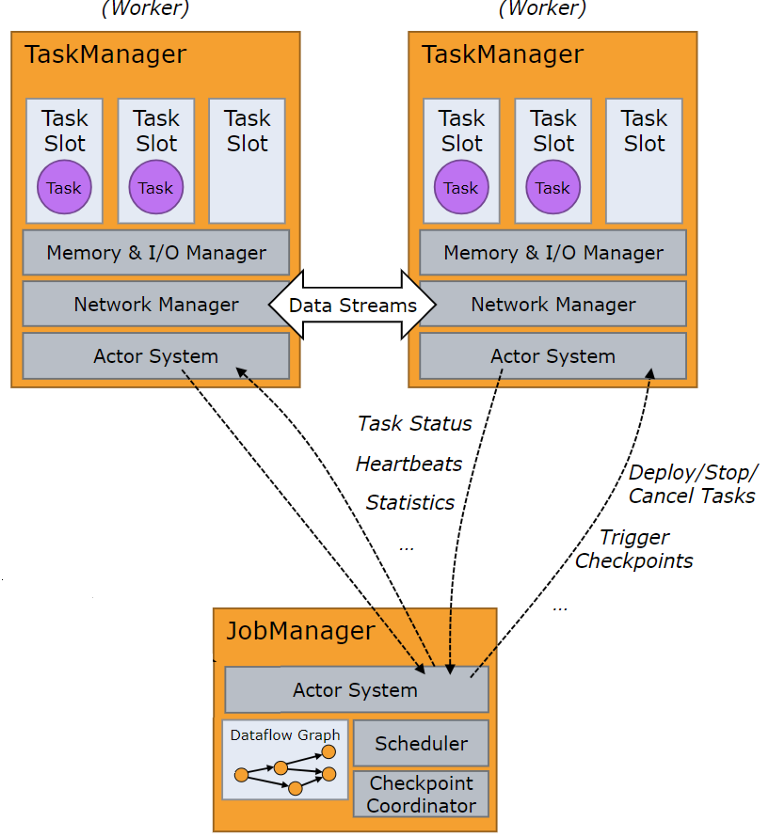
\includegraphics[width=0.9\textwidth]{img/flink_technical_archi}
    \captionof{figure}{Apache Flink technical architecture}
\end{center}

%continue editing from here

\subsection{Components of a Flink cluster}

\subsubsection{JobManager}
The JobManager is the brain of our Flink cluster.
It has several responsibilities related to the coordination of distributed execution of Flink applications: it decides when to schedule the next task (or set of tasks), reacts to completed tasks or execution failures, coordinates checkpoints and recovery in case of failure, among others.
This process consists of three different components:

\begin{itemize}
    \item \textbf{ResourceManager:} It is responsible for the de-/allocation and provisioning of resources in a Flink cluster.
    \item It manages task slots, which are the unit of resource scheduling in a Flink cluster.
    \item Flink implements several ResourceManagers for different environments and resource providers such as YARN, Kubernetes, and standalone deployments.
    \item In a standalone configuration, the ResourceManager can only distribute the slots of available TaskManagers and cannot start new ones by itself.
    \item \textbf{The Dispatcher:} The Dispatcher provides a REST interface to submit Flink applications for execution and starts a new JobMaster for each submitted job.
    \item It also runs the Flink WebUI to provide information about job executions.
    \item \textbf{The JobMaster:} The JobMaster is responsible for managing the execution of a single JobGraph.
    \item Multiple jobs can run simultaneously in a Flink cluster, each having its own JobMaster.
\end{itemize}

There is always at least one JobManager.
A high-availability configuration can have multiple JobManagers, one of them always being the leader, and the others being on standby.

\subsubsection{TaskManager}
TaskManagers (also called Workers) execute the tasks of a data stream, exchanging information through buffer memory.
TaskManagers are responsible for the effective execution of data processing operations.
They manage read, transformation, and write operations within a Flink cluster.
There must always be at least one TaskManager.

The smallest unit of resource scheduling in a TaskManager is a task slot.
The number of task slots in a TaskManager indicates the number of simultaneous processing tasks.
One or more parallel instances of an operation can run in the same Task Slot.

Operations to be executed are divided into sub-tasks, depending on the default or specified parallelism options.
One or more parallel instances of an operation are carried out in a Task Slot.
The Task Slot represents an isolated memory space dedicated to the execution of one or more processing threads.
A TaskManager can have one or more Task Slots.

Each TaskManager sends a heartbeat message at regular intervals and receives them from the JobManager to signal that it is not down.
If a TaskManager fails, the JobManager redistributes tasks among the operational TaskManagers by resuming the job from the last completed checkpoint.

\begin{center}
    \centering
    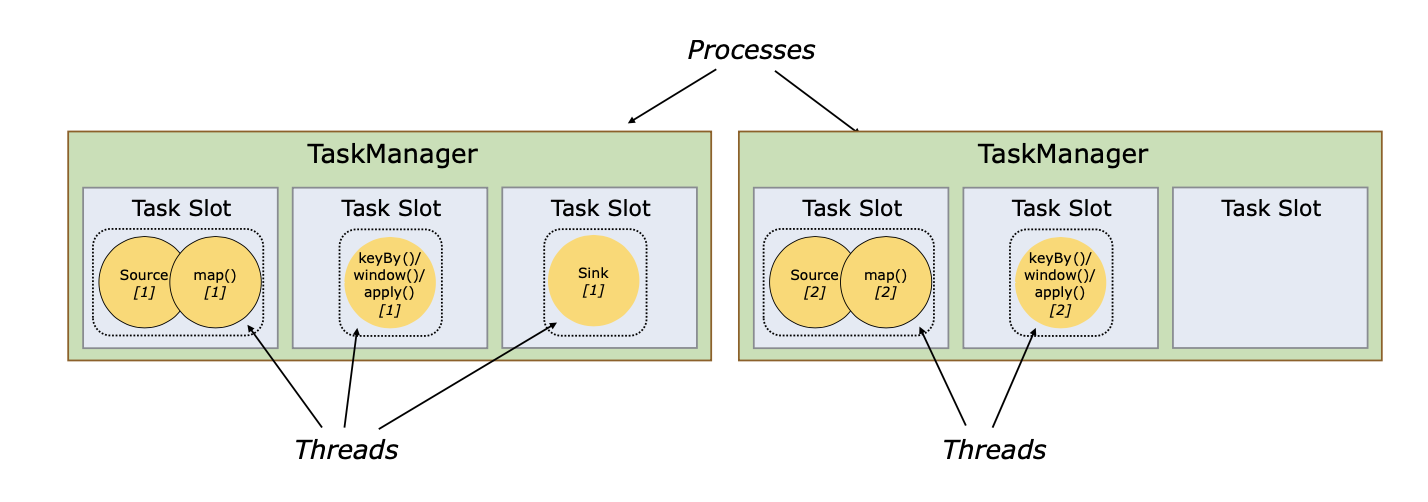
\includegraphics[width=1\textwidth,height=6cm]{img/task_slots}
    \captionof{figure}{Task slots}
\end{center}

\subsection{Job scheduling}
A Flink job is first in the \textit{created} state, then it is \textit{running}, and once its work is complete, it is \textit{finished}.
In case of failure, the job transitions to \textit{failing} and cancels all currently running tasks.
If all job vertices have reached the final state and the job cannot be restarted, the job has \textit{failed}.
If the job can be restarted, it will transition to the \textit{restarting} state.
Once the job has been restarted, it will reach the \textit{created} state.
If the user cancels the job, it will transition to the \textit{cancelling} state.
This also involves cancelling all currently running tasks.
Once all running tasks have reached the final state, the job transitions to the \textit{cancelled} state.
Unlike the \textit{finished}, \textit{cancelled}, and \textit{failed} states which denote a global terminal state and thus trigger job cleanup, the \textit{suspended} state is only locally terminal.
Locally terminal means that the job execution has ended on the respective JobManager, but another JobManager in the Flink cluster can retrieve the job from the persistent high-availability storage location and restart it.
Therefore, a job that reaches the \textit{suspended} state will not be completely cleaned up.

\begin{center}
    \centering
    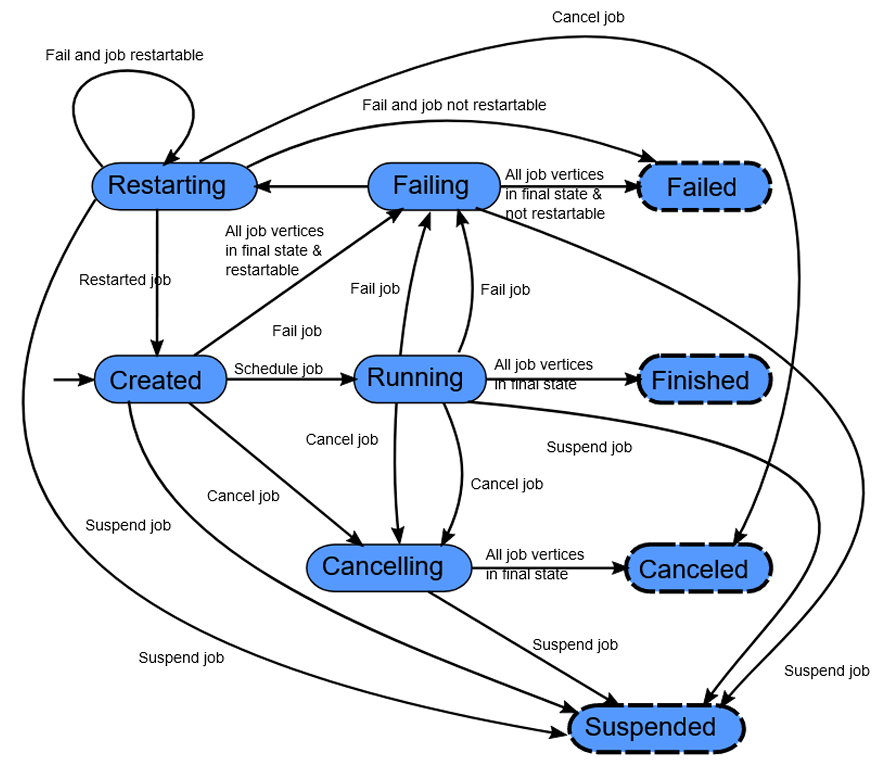
\includegraphics[width=0.9\textwidth]{img/job_scheduling}
    \captionof{figure}{Job scheduling}
\end{center}

\subsection{Fault tolerance}

\subsubsection{Checkpointing}
One of Flink's strengths is its checkpointing mechanism.
This mechanism consists of taking automatic and asynchronous snapshots of the application state and position in the stream at regular intervals.
This provides the guarantee that each piece of data is processed exactly once (exactly-once processing delivery guarantee) with low performance impact.

In case of failure or breakdown, a Flink program with checkpoints enabled will resume processing from the last checkpoint, ensuring that Flink maintains processing uniqueness.
The checkpoint mechanism can also be extended to writing and reading from a database.

Flink allows the user to manually trigger checkpoints; these are then called savepoints and allow, for example, stopping the program and resuming from the saved state, or restarting the application with different parallelism to adapt to changes in stream speed and volume.

\begin{center}
    \centering
    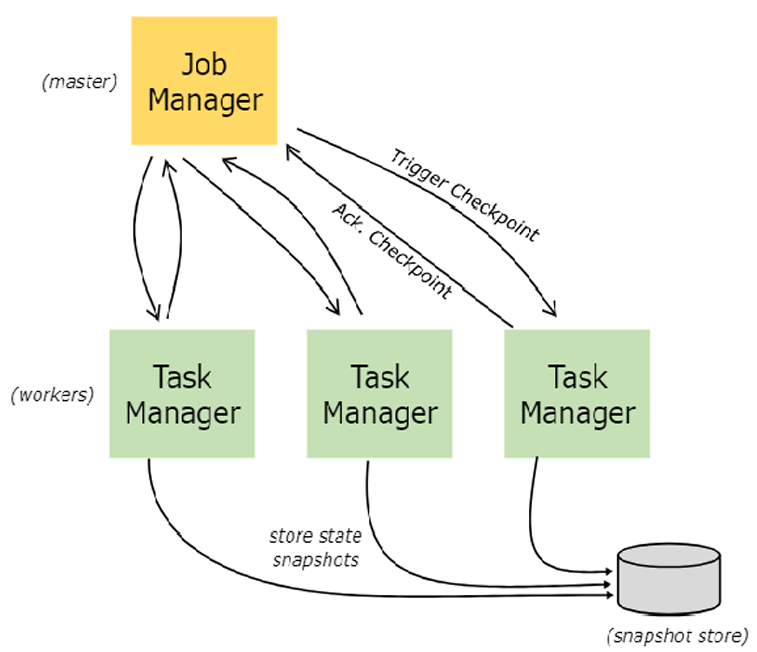
\includegraphics[width=0.9\textwidth]{img/checkpointing}
    \captionof{figure}{Checkpointing mechanism}
\end{center}

\subsubsection{JobManager high availability}
The drawback of this type of architecture is the uniqueness of the master, which represents a single point of failure (SPOF), since by default, a Flink cluster contains a single JobManager.
If the JobManager fails, the TaskManagers notice because they are disconnected from the JobManager, but there is no procedure for electing a new JobManager among them (TaskManagers remain slaves).
To mitigate this risk, Flink offers a procedure called High Availability.
The idea is to have a leader JobManager and one or more standby JobManagers, ready to take over if the leader fails or becomes unavailable.
Typically, this procedure is handled by a widely used underlying framework, ZooKeeper.
However, using high availability with ZooKeeper on Kubernetes incurs additional costs, as we must manage a ZooKeeper cluster.
On the other hand, Kubernetes provides a public API for leader election and configuration storage (e.g., ConfigMap).
We can leverage these features to make running a Flink cluster configured for high availability on Kubernetes more practical.

\begin{center}
    \centering
    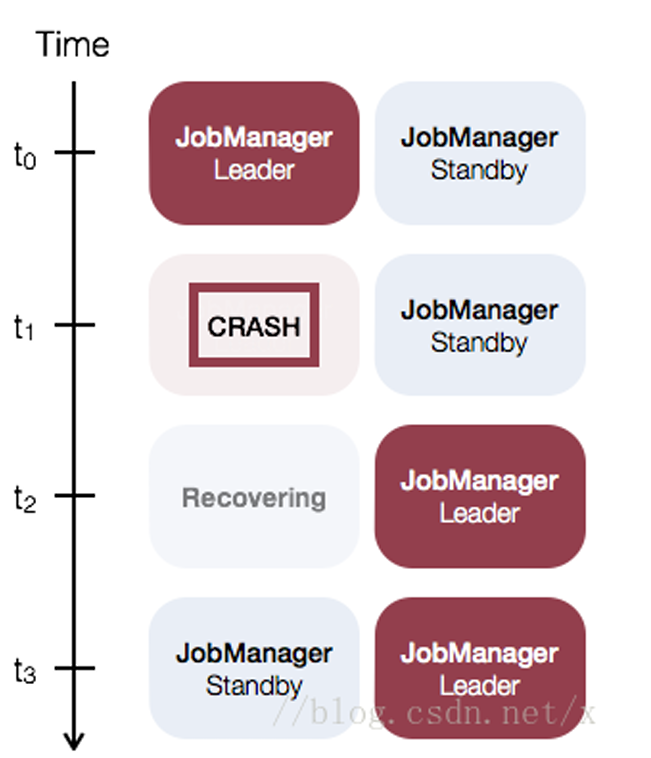
\includegraphics[width=0.8\textwidth,height=10cm]{img/ha_jobmanager}
    \captionof{figure}{JobManager high availability management mechanism}
\end{center}

\subsection{Security}
When securing network connections between machine processes via authentication and encryption, Apache Flink distinguishes between internal and external connectivity.
Internal Connectivity refers to all connections established between Flink processes.
These connections run Flink's custom protocols.
Users never connect directly to internal connectivity endpoints.
External Connectivity refers to all connections established from outside to Flink processes.
This includes the Web UI and REST commands to start and control running Flink Jobs, including communication from the Flink CLI with the Job Manager/Dispatcher.
For greater flexibility, internal and external connectivity security can be enabled and configured separately.

\begin{center}
    \centering
    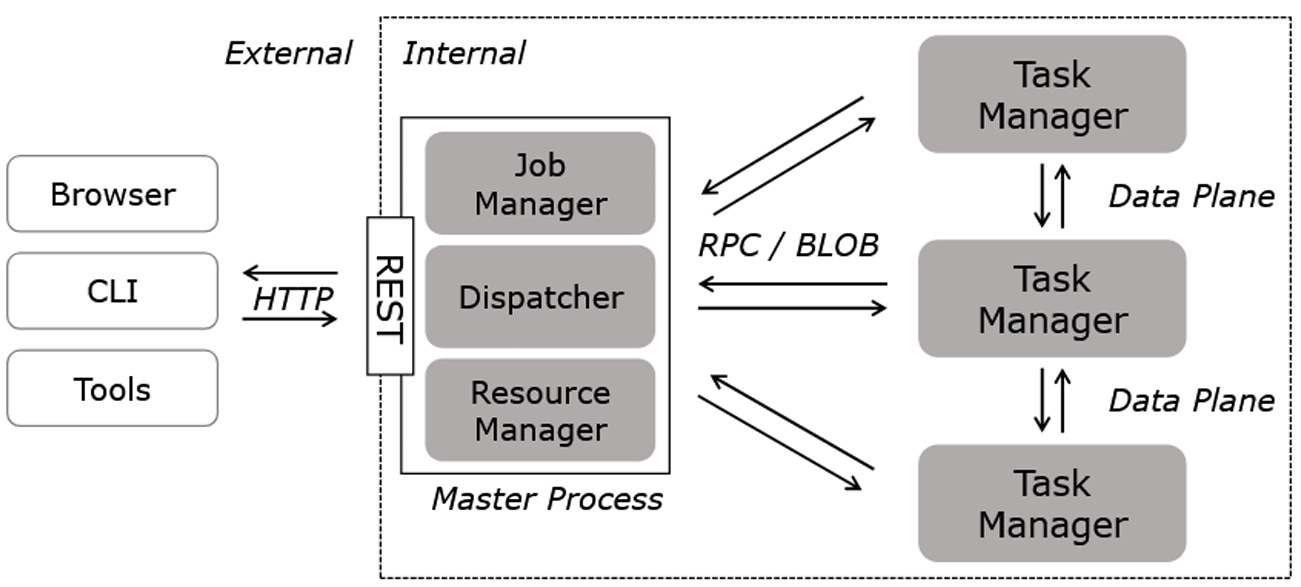
\includegraphics[width=0.9\textwidth]{img/flink_connectivity}
    \captionof{figure}{Connectivity}
\end{center}

\subsubsection{Internal connectivity}
Internal connectivity includes:
\begin{itemize}
    \item \textbf{Control messages:} RPC between Job Manager / Task Manager / Dispatcher / Resource Manager.
    \item \textbf{Data plane:} Connections between Task Managers for exchanging data during shuffling, broadcasting, redistribution, etc.
    \item \textbf{Blob service:} Distribution of libraries and other artifacts.
\end{itemize}

All internal connections are SSL-authenticated and encrypted.
Connections use mutual authentication, meaning that both the server and the client of each connection must present their certificate to each other.
The certificate effectively acts as a shared secret.

\subsubsection{External connectivity}
All external connectivity is exposed via an HTTP/REST endpoint, used for example by the Web interface and the CLI:
\begin{itemize}
    \item Communication with the Dispatcher to submit jobs (session cluster).
    \item Communication with the Job Manager to inspect and modify a running job/application.
\end{itemize}

REST endpoints can be configured to require SSL connections.
However, the server will accept connections from any client by default, meaning the REST endpoint does not authenticate the client.

